\documentclass[12pt]{article}
\usepackage{graphicx}
\usepackage{subcaption}
\usepackage{tikz}

\pagestyle{empty}
\begin{document}
\begin{figure}
\centering
\begin{subfigure}{.073\textwidth}
    \centering
    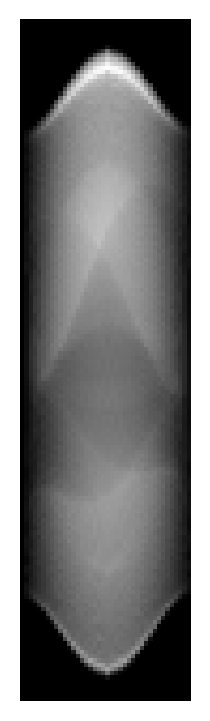
\includegraphics[width=\textwidth]{../figures/data-full.png}
\end{subfigure}%
\begin{subfigure}{.25\textwidth}
    \centering
    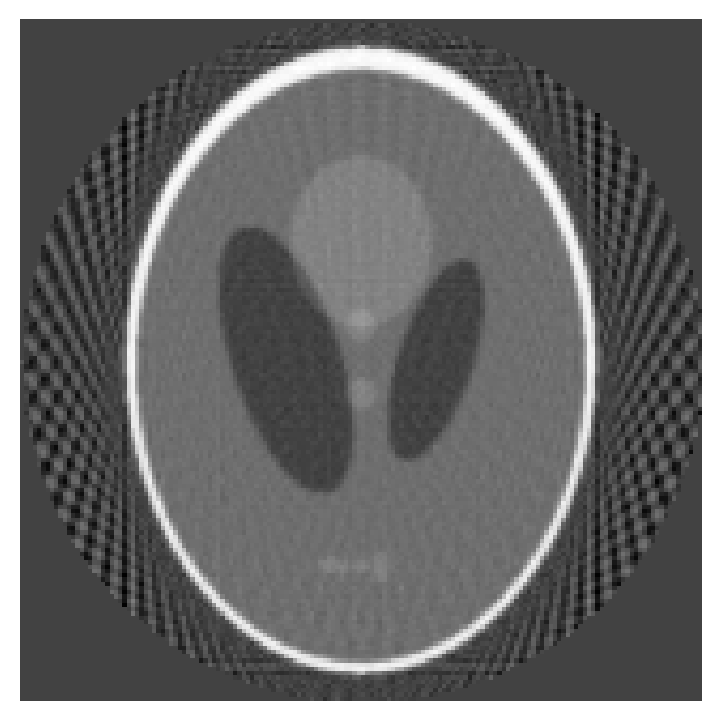
\includegraphics[width=\textwidth]{../figures/FBP-full.png}
\end{subfigure}
\begin{subfigure}{.25\textwidth}
    \centering
    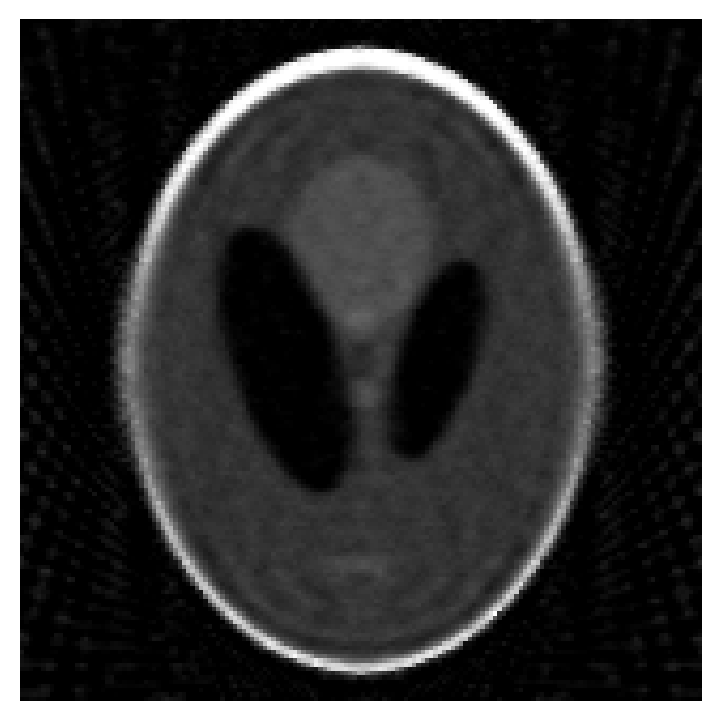
\includegraphics[width=\textwidth]{../figures/TV-full.png}
\end{subfigure}%
\begin{subfigure}{.25\textwidth}
    \centering
    
\includegraphics[width=\textwidth]{../figures/GT.png}
\end{subfigure}\\
\begin{subfigure}{.073\textwidth}
    \centering
    
\includegraphics[width=\textwidth]{../figures/data-half.png}
\end{subfigure}%
\begin{subfigure}{.25\textwidth}
    \centering
    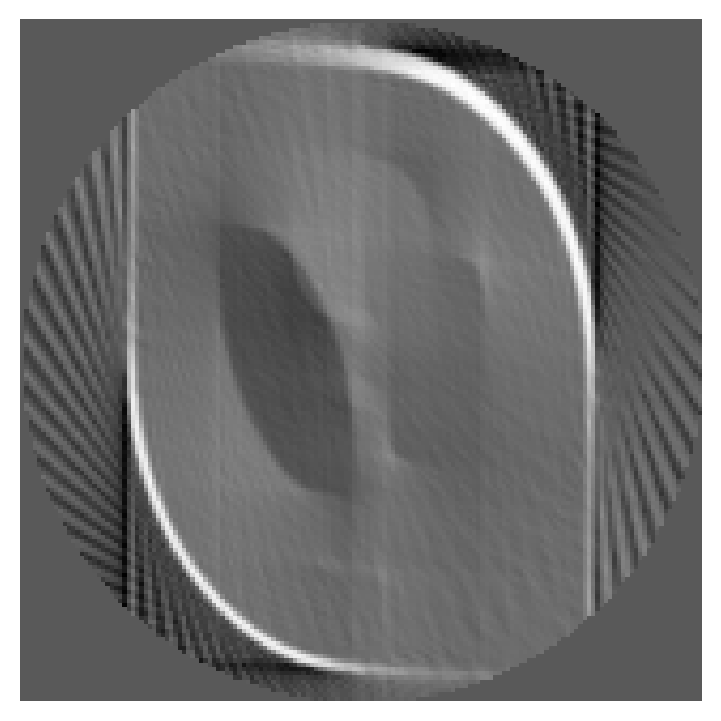
\includegraphics[width=\textwidth]{../figures/FBP-half.png}
\end{subfigure}
\begin{subfigure}{.25\textwidth}
    \centering
    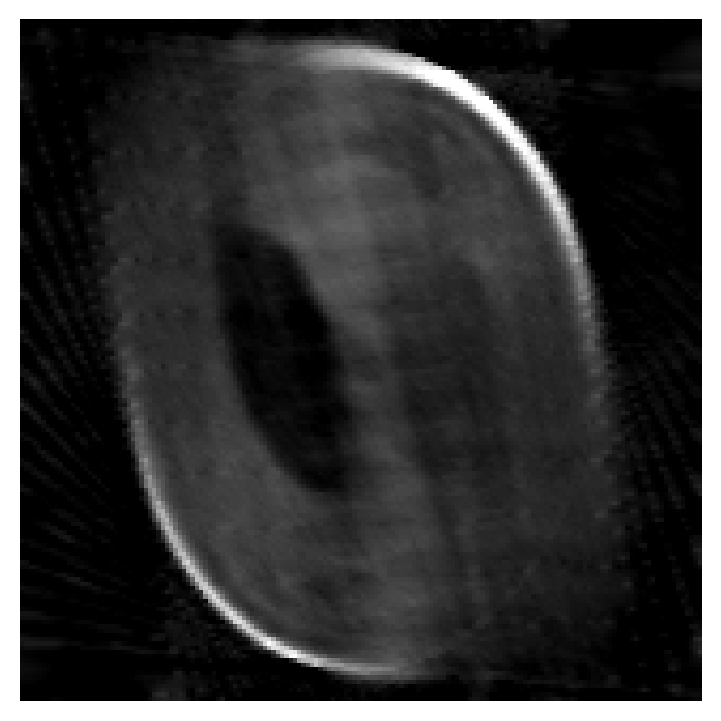
\includegraphics[width=\textwidth]{../figures/TV-half.png}
\end{subfigure}%
\begin{subfigure}{.25\textwidth}
    \centering
    
\includegraphics[width=\textwidth]{../figures/GT.png}
\end{subfigure}%
\label{fig: experiments}
\end{figure}%
\end{document}

